\documentclass[acmtog, authorversion]{acmart}

\usepackage{booktabs} % For formal tables

\usepackage[ruled]{algorithm2e} % For algorithms
\renewcommand{\algorithmcfname}{ALGORITHM}
\SetAlFnt{\small}
\SetAlCapFnt{\small}
\SetAlCapNameFnt{\small}
\SetAlCapHSkip{0pt}
\IncMargin{-\parindent}

% Metadata Information
% \acmJournal{TOG}
% \acmVolume{9}
% \acmNumber{4}
% \acmArticle{39}
% \acmYear{2010}
% \acmMonth{3}

% Copyright
%\setcopyright{acmcopyright}
%\setcopyright{acmlicensed}
%\setcopyright{rightsretained}
%\setcopyright{usgov}
\setcopyright{usgovmixed}
%\setcopyright{cagov}
%\setcopyright{cagovmixed}

% DOI
% \acmDOI{0000001.0000001_2}

% Paper history
% \received{February 2007}
% \received{March 2009}
% \received[final version]{June 2009}
% \received[accepted]{July 2009}


% Document starts
\begin{document}
% Title portion
\title{Phenotype Prediction from Human Whole Genome Profile}
\author{Mengying Sun}
\orcid{1234-5678-9012-3456}
\affiliation{%
  \institution{Michigan State University}
  \department{Department of Computer Science and Engineering}
  \streetaddress{TBD}
  \city{East Lansing}
  \state{MI}
  \postcode{00000}
  \country{USA}}
\author{Xiaoran Tong}
\affiliation{%
  \institution{Michigan State University}
  \department{Department of Epidemiology and Biostatistics}
  \streetaddress{909 Fee Rd}
  \city{East Lansing}
  \state{MI}
  \postcode{48824}
  \country{USA}
}

\renewcommand\shortauthors{Zhou, G. et al}

\begin{abstract}
  Through this project we seek to predict complex human phenotype from high dimensional whole genome profiles. To solve the curse of dimensionality, we adopted a two tier modeling by first choosing representative features from chromosome LD blocks, then build a higher tier predictive model upon the first tier output. We expect improvement of predictive accuracy over existing GWAS or kernel based models.
\end{abstract}


%
% The code below should be generated by the tool at
% http://dl.acm.org/ccs.cfm
% Please copy and paste the code instead of the example below. 
%
% \begin{CCSXML}
% <ccs2012>
%  <concept>
%   <concept_id>10010520.10010553.10010562</concept_id>
%   <concept_desc>Computer systems organization~Embedded systems</concept_desc>
%   <concept_significance>500</concept_significance>
%  </concept>
%  <concept>
%   <concept_id>10010520.10010575.10010755</concept_id>
%   <concept_desc>Computer systems organization~Redundancy</concept_desc>
%   <concept_significance>300</concept_significance>
%  </concept>
%  <concept>
%   <concept_id>10010520.10010553.10010554</concept_id>
%   <concept_desc>Computer systems organization~Robotics</concept_desc>
%   <concept_significance>100</concept_significance>
%  </concept>
%  <concept>
%   <concept_id>10003033.10003083.10003095</concept_id>
%   <concept_desc>Networks~Network reliability</concept_desc>
%   <concept_significance>100</concept_significance>
%  </concept>
% </ccs2012>  
% \end{CCSXML}

% \ccsdesc[500]{Computer systems organization~Embedded systems}
% \ccsdesc[300]{Computer systems organization~Redundancy}
% \ccsdesc{Computer systems organization~Robotics}
% \ccsdesc[100]{Networks~Network reliability}

%
% End generated code
%

% We no longer use \terms command
\terms{AI, Algorithms, Performance}

\keywords{ReLU}


\thanks{This work is supported by the National Science Foundation,
  under grant CNS-0435060, grant CCR-0325197 and grant EN-CS-0329609.

  Author's addresses: G. Zhou, Computer Science Department, College of
  William and Mary; Y. Wu {and} J. A. Stankovic, Computer Science
  Department, University of Virginia; T. Yan, Eaton Innovation Center;
  T. He, Computer Science Department, University of Minnesota; C.
  Huang, Google; T. F. Abdelzaher, (Current address) NASA Ames
  Research Center, Moffett Field, California 94035.}


\maketitle

\newcommand{\bs}[1]{\boldsymbol{#1}}
\section{Introduction}
The prediction of complex phenotype from whole genome profile is still far from satisfactory, leaving large gaps between empirical heritability measured by classic pedigree studies and contemporary kernel based whole genome predictive methods that pools huge number of features across the entire genome \cite{WGP:Gustavo, WGP:Zhang, GCTA, WGP:GMatrix1, WGP:Review1}. Among popular proposals, some attribute the ``missing heritability'' to violation of the overly strong assumption that genomic effect are additive, that is, phenotype y is linked to the linear combination of genomic features $G$ or limited expansion $\bs{\phi}(G)$. The violation of linearity and between feature independence are frequently violated, demonstrable by association rules detected by screening tuple of features combinations \cite{GWA:GMDR, GWA:MDR}. To tackle non-linearity and feature combinations into prediction modeling, the recent trend of machine learning suggests multi-layered neural network (NN) that regained popularity around 2006 through a pre-training procedures \cite{DL:Intro1}, and pushed to a new depth by replacing the classical sigmoid activation to rectified linear unit (ReLU) \cite{DL:Relu1}. However, a typical NN for genomic prediction is computationally intractable due to the sheer size of the profile easily breaching the order of tens of millions features thanks to the next generation sequencing technology \cite{NGS1}.

To construct NN predictor on genomic profiles, it is desirable to design dimensionality reduction prior to train the whole genome NN. A widely practices technique in the field of whole genome association studies (GWAS) is to drop the bulk of rare or extremely rare features in the population, that is, only a handful of individuals has non-zero values in nearly 90\% of the features. Even after such selection, the size of the profiles are till in the order of millions. Another useful characteristic of genome is that features closely located in a chromosome segment are highly correlated due to the chemical bounds between nucleotides - a phenomenon known as linkage disequilibrium (LD) \cite{LD:Intro1, LD:Haploview}. More formally, LD states that the frequency of observing a particular type of feature variation at one site is not independent to the joint configuration observed at some other sites, and such reliance grows with proximity of the sites. As a result, there is a nature division of the genome into several thousands to tens of thousands of LD blocks, such that features in a block are significantly more correlated than those between blocks. Each LD block can then be represented by a small number of selected or extracted feature since high correlation suggest high redundancy. Thus, by exploiting the genomic LD structure, the complexity of the prediction may be divided and conquered through separately reducing the dimensionality of each block, followed by training the predictor upon the intermediate feature of much lower dimension.

In this study we aim to predict the standard phenotype - body height with features through out the whole genome. We propose a two tier approach that identify LD blocks and select/extract features from each block at the first stage, and train the predictive model on the selected/extracted few features at the second stage. With both real and simulated phenotype, we put a variety of feature selection, feature extraction, and neural network configurations through benchmarks. We assume that by using neural network to model the non-linear feature-phenotype association and feature-feature interactions, the two tier predictor should outperform contemporary product kernels based whole genome prediction methods \cite{WGP:Gustavo} and linear feature extraction method such as principle component analysis (PCA). This assumption is to be tested via benchmarks as well.

Regarding the training of NN for both tier one feature extraction and tier two predictor, the current norm taken from machine learning field is the pursuit of deeper networks, which indeed scored many victories in the last decade\cite{DL:Intro2, DL:Intro3}. However, the central doctrine that ``deeper is better'' may no longer hold true when the question domain shifts from visual, acoustic and text data into genomes, considering its innate sparsity and categorical nature. This study also aims to find out suitable type and depth of the NN specifically for the genome data, through large number of benchmarks.

\section{Material}
The body height target variable and the corresponding whole genome profiles were obtained from UK Bio-bank \cite{Data:UK_Biobank}, a prospective cohort study of over 500K individuals from across the United Kingdom during 2006 and 2010. In our study, the genomic variables are exclusively single nucleotides polymorphisms (SNPs). A total of 589,028 SNP readings for 102,110 individuals passed the following quality control: (i) removal of SNPs with MAF (minor allele frequency) < 0.05, that is, genome sites of rare variation; (ii) removal of SNPs with missing values in more than 30\% of the participants; (iii) removal of individuals with incomplete mapping between phenotype and genomic profiles. To evaluate generalization performance, we split data into training and testing set, with 80,000 observations for training and 22,110 for testing. 

For simulation studies, only genomic data is required. We draw 503 Whites of European origin from 1000 genome project \cite{Data:1K_Genome} provided by National Center for Biotechnology Information (NCBI). The actual sample size is achieved by repetitively sampling from the 503 genotype with replacing. After removing rare features, a total of 6,937,859 features remained in the study.

All genomic features correspond to variable sites comprising less than 1 percent of the human genome. A features is is coded as minor allele count of the corresponding site, usually called dosage value. A feature gets 0 dosage if both homogeneous chromosomes at that site concord the reference genome constructed from 14 volunteers from New York; conversely, it gets a dosage value 1 or 2, if one, or both chromosomes at that site are different from the reference. A genome profile can then be seen as an ultra high dimensional vector that takes discrete values in $\{0, 1, 2\}$.

To identify LD blocks, we use population genetic package PLINK2.0 \cite{PK:Plink2}, which produces subsets of features that are in approximate linkage disequilibrium (LD) with each other. It is based on correlations between genotype allele counts. Two features are considered to be in strong LD if the bottom of the 90\% $D\prime$ confidence interval is greater than 0.70, and the top of the confidence interval is at least 0.98. For now, only pairs of variants within 400 kilo-bases of each other are considered. For UK Biobank data, a total of 190,174 LD-blocks were identified using these criteria, for the 1000 genome data, the number is [?]. Due to many generations of genome recombination during reproduction, most some LD blocks come small in size, to facilitate certain feature selection/extraction methods, we combined consecutive LD-blocks to form super-blocks of relatively large and stable number of raw features, knowing that the correlation between super-blocks are still relatively small.

\section{Method}
\subsection{Tier one}
This stage of modeling divide the genome into relatively unrelated block and perform selection or extraction of intermediate features from the blocks.
\subsubsection{Supervised Feature Selection}
To achieve supervised genomic feature selection, first we perform a genome-wide association study (GWAS) for the training data set. In GWAS, we regress height on each marker using simple linear regression, with p-value generated and adjusted to $-log(10)$ scale. Large adjusted p-value indicates strong association between response and the marker. GWAS was done by “BGData” package in R. Results can be found at Figure \ref{gwas}. The transformed p-values are shown in the genomic Manhattan plot below:
\begin{figure}[h]
  \centering
  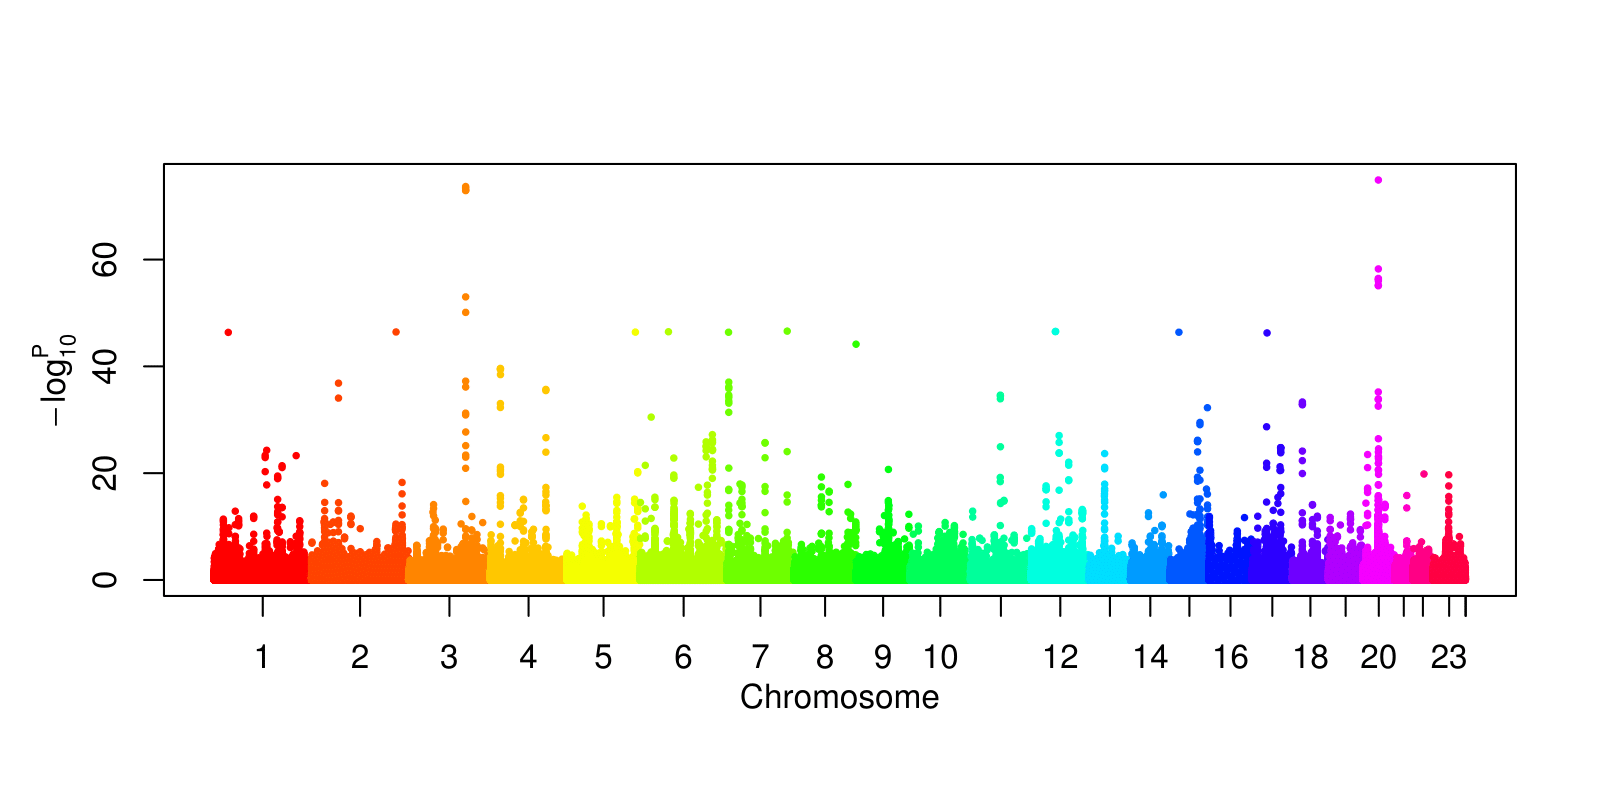
\includegraphics[width=3.5 in, trim=0 0 0in 0]{img/gwas_height}
  \caption{Negative log p-value for 600K markers.}
  \label{gwas}
\end{figure}

Feature selection was done through four different approaches: (i) top-k selection, in which we ordered adjusted p-values in descending order in a global sense and select top k markers across whole genome; (ii) step-wise selection based on Bayesian information criteria (BIC) for each block; (iii) selection based on LASSO in each block. (iv) Randomly choose features across whole genome for control purpose. 

For step-wise selection, it is possible that a block ends up with no feature selected, which implies we discard the whole block. For LASSO selection, since many blocks contains only one feature which makes it meaningless to implement lasso, we merge consecutive blocks to super blocks with length around 300 features per block. Then we implement lasso on the super block. For each block, we divide the training set into sub-training and sub-validation set. We first calculate the solution path for $w$ with respect to $\lambda$ in sub-training set, and choose $\lambda$ such that the correlation between $y$ and $\hat{y}$ is maximized in sub-validation set. Then we apply this $\lambda$ in the whole training set to get the estimates for each feature. In case that the dimension are still high after selecting non-zero coefficients, we also output a score for each block based on estimates. Step-wise selection was done using base function Set() in R and lasso selection was done using the clement package in R [ref].

Summary for selections can be found at Figure {\ref{fig:BIC}}. We got 6022 selected SNPs in 5554 blocks. For lasso we get more than 20000 non-zero effects thus we maintain a score of each block and end up with 1867 scores. In order fro comparing between different selection methods, we choose 6022 features with largest adjusted p-value for the top-p selection and 6022 random features for control case.
% \begin{figure}[!h]
%   \centering
%   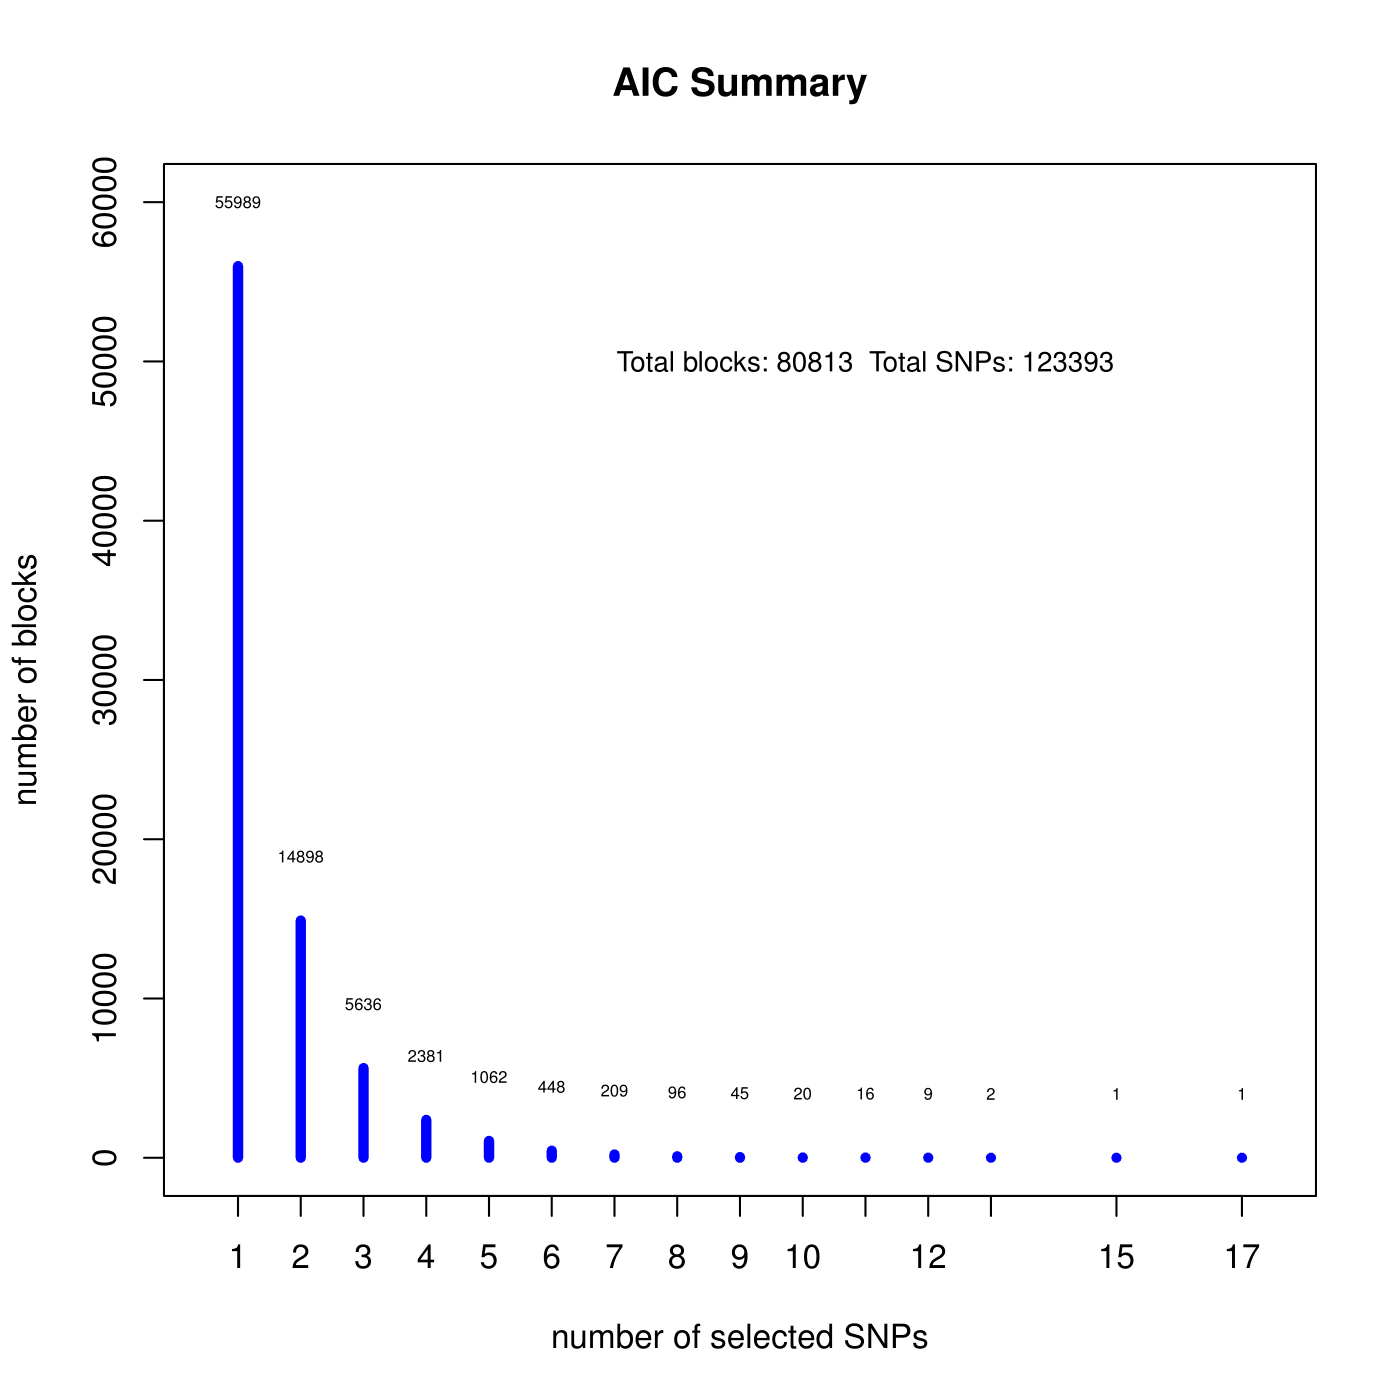
\includegraphics[width=3.5 in, trim=0 0 0in 0]{img/AIC_summary}
%   \caption{Variable selection by AIC}
%   \label{fig:AIC}
% \end{figure}
\begin{figure}[!h]
  \centering
  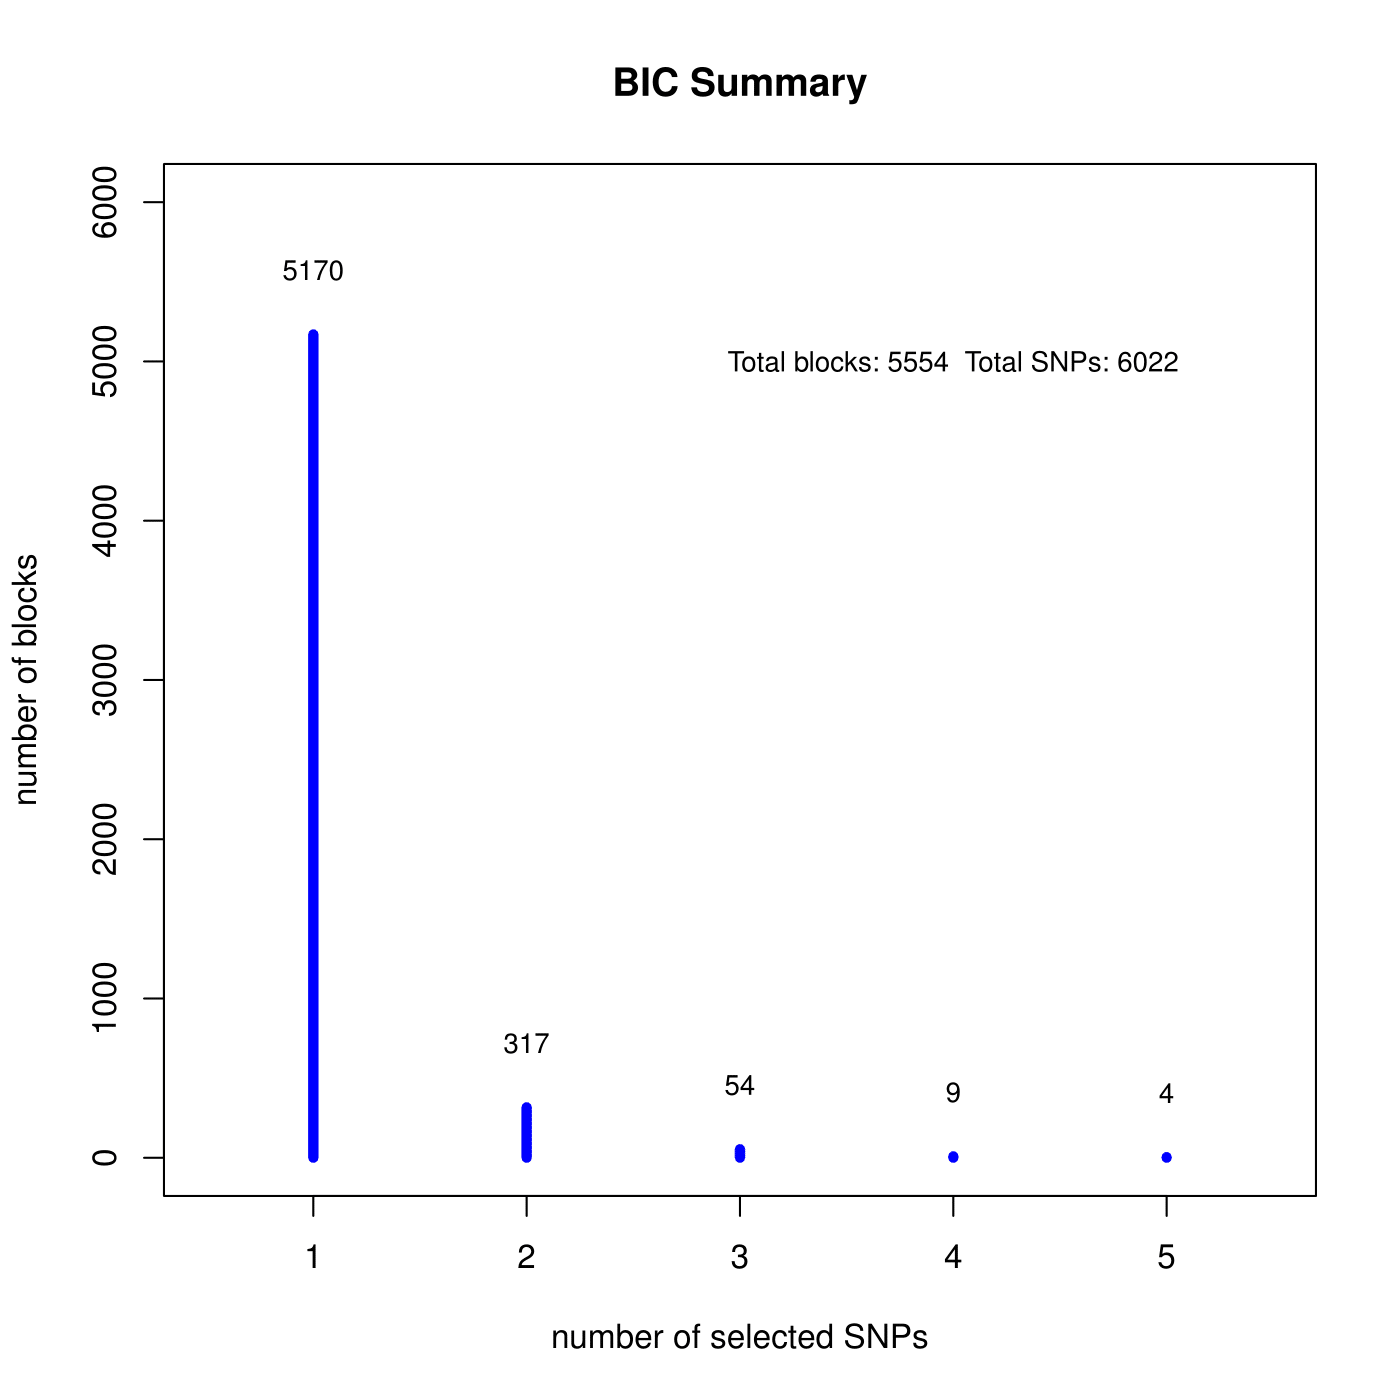
\includegraphics[width=3.5 in, trim=0 0 0in 0]{img/BIC_summary}
  \caption{Variable selection by BIC}
  \label{fig:BIC}
\end{figure}


\subsubsection{Unsupervised Feature Extraction}
We choose stacked autoencoder(SA) \cite{DL:SDA1} to preserve non-linearity when extracting on high order feature from each super-block containing roughly 1000 raw feature. To facilitate the training, and also relax the additive genetic effect assumption, features taking count value in $\{0, 1, 2\}$ are flattened by lining up the two homogeneous chromosomes, which ends up with a double sized binary vector. At this stage we seek to overfit the encoder in pursuit of maximum preservation of genomic signal.

Before actual training and feature extraction, we benchmark the performance of sigmoid and ReLU SAs with randomly chosen genome segments of $512$ features ($1024$ after flattening) without considering LD, which is intended to find out configuration better suited for genome related tasks. The performance is gauged by training error given the same budget of epochs without early stop, weight decay, and denoising.

The current setting halves the dimension with increasing depth, until the output become one dimensional, which gives up $1024, 512, \dots, 2, 1$ nodes in a 10 layered encoder. Both sigmoid and ReLU activation are tested (except the last reconstruction layer always use sigmoid to restore binary feature). The mean performance of 1000 trails is shown in Figure (\ref{fig:ae0}).
\begin{figure}[h]
  \centering
  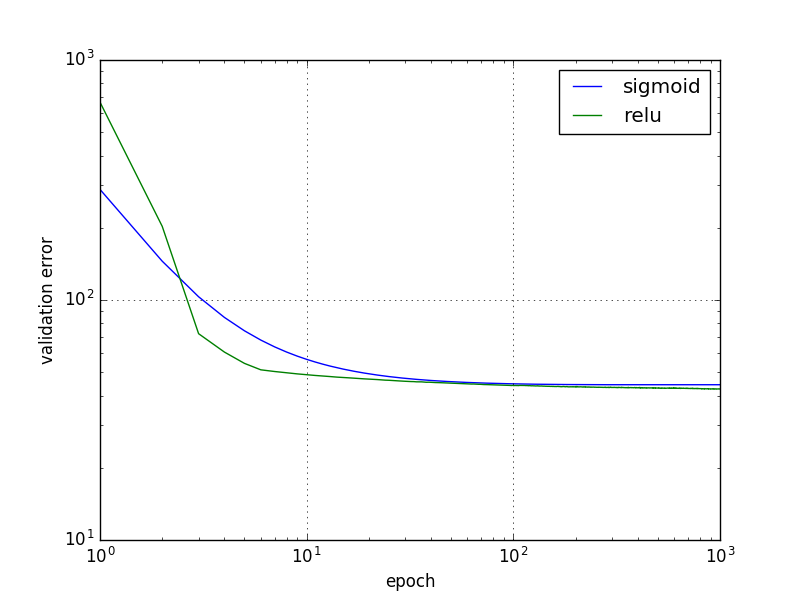
\includegraphics[width=0.35\textwidth]{img/00}
  \caption{Autoencoder Test, depth=10}
  \label{fig:ae0}
\end{figure}
The  ReLU activation maintained a small edge over sigmoid networks even after long period of training, it also converge faster as suggested \cite{DL:Relu1}. However, the sigmoid networks did not go through the suggested layer-wise pre-train \cite{DL:Intro1} in order to make the benchmark comparable. The sigmoid activation may perform as good as ReLU for a shallow SA of $10 \time 2$ layers if pre-training was done. On the other hand, ReLU suffers from numerical instability due to the drastic change intermediate layers that leads to overflow, because a stack of 10 autoencoders is not deep enough to diminish the gradient that drives network change. To reduce the chance of overflow below \%0.5, we have set initial learning rate to a value as low as 1e-6, which defeat the advantages of fast convergence brought by ReLU. Deeper SA network may justify the use of ReLU, but they failed to further lower the training error while demanding a significantly increase in running time. 

We decide classical sigmoid activation for the SAs, also implement pre-training to drive down reconstruction loss. A total of 6122K super-blocks of roughly 1K raw features were ``encoded'' to produce a $6122$ dimensional vector $\bs{h}_1$ holding input features for tier two models. To train such a large number of SAs, a few powerful GPU node is not feasible, we rely on slower but much more numerous CPU nodes on MSU HPCC instead, together with a much richer wealth of secondary storage which we could implement the bold driver heuristics to trade off for some compensation in processing speed.

To test the aforementioned hypothesis of ``missing heritability'', we applied principle component analysis(PCA) on the super-blocks as well, and pick out the largest PC of each to form another intermediate feature vector $\bs{h}_1^{\prime}$ as the control of $\bs{h}_1$, knowing that PCA is pure linear transformation. If the hypothesis holds true, the tier two model trained with $\bs{h}_1$ should work better than $\bs{h}_1^\prime$, which will be put into test by the simulation studies.

\subsection{Tier Two: Predictive Model}
Currently the high data analysis is only based on feature selection at tier one. We consider two types of prediction models: i) Bayesian generalized linear models (as control); ii) Neural networks (as proposal). We feed selected features into these two types of models and see the prediction performance.

\noindent \textbf{Bayesian generalized linear models} \\
BGLM assumes the effects follows a prior distribution, and estimates them by sampling from the posterior distribution of those effects. Different prior corresponds to different regularization in optimizing the loss function characterized by residual sum of squares. A ridge regression assuming Gaussian prior is equivalent to $l_2$ norm constraint, and a Laplacian prior is equivalent to $l_1$ norm penalty known as lasso. In our case, we tried ``BayesB'' which assigns two component mixture prior with a point of mass at zero and a scaled-t slab. This prior is demonstrated to have best performance in previous peer work. All the analysis for this method was done using the ``BGLR'' package in R [ref]. 

\noindent \textbf{Neural Network} \\
So far the commonly used models for genomic prediction assumes that the genetic effects are linear. Whether there is nonlinear effects and whether we can capture those nonlinear effects using other methods are still an open question. With the rapidly developed techniques such as neural networks in computer science society, and due to it’s highly nonlinear structure and property, it is possible that some nonlinear patterns of genetic effects can be found. Therefore we decide to build such a framework to evaluate the effects for height trait.

The network is built in Keras [ref], we implemented two hidden layers for the network with the first layer reduces input features to a dimension of 256, and second layer reduce feature dimension to 16. Next, we choose different settings for the network to see how each component affects our results. The process is as following: i) different activation functions; ii) different learning rate; iii) different sample size; iv) different regularization parameters. At last, we implement our network by using the tuned settings to evaluate our performance. 

\subsection{Simulation Study}
The simulation study uses extracted features only, which is based the 1000 genome project data \cite{Data:1K_Genome}. The main performance comparison happens between NN trained using $\bs{h}_1$ -- the intermediate feature produce by SAs, and $\bs{h}_1^\prime$ produced by linear PCA.

Each simulation instance starts with randomly sampling $P$ features (without replacement) and $N$ data points from the genome pool of 503 White Europeans (with replacement), call it $\bs{X}^{N \times P}$. For now $P$ is one hundredth of the total of 7 million features. We then assign the $P$ features with genetic scores $\bs{w} $drawn from $N(\bs{0}, \bs{1}^{P \times P})$. Two sets of genetic effect may be simulated, either a simple additive effect with no manipulation of feature values which should favor the PCA generated $\bs{h}_1^\prime$, or an composition three effects: Additive, Dominant, and Recessive done by masking out part of the features, which is more biologically plausible. The genomic signal for each individual is the inner product between his/her features ($\bs{x}_i$, possibly masked), and the assigned genetic scores ($\bs{w}$), that is
\begin{align*}
  \eta_i =
  \begin{cases}
    \bs{w}^T \bs{x}_i                                                                & \textrm{(Only Additive)} \\
    \bs{w}^T [\alpha\bs{x}_i + \beta I_{\bs{x_i} \ne 0}  + \gamma I_{\bs{x_i} = 2}], & \textrm{(Composition)}
  \end{cases}
\end{align*}
where $\alpha + \beta + \gamma = 1$ give the proportion of additive, dominant and recessive genetic effect.
At this point some noise is drawn from $N(\bs{0}, \bs{1}^{N \times N})$ to obscure the true signals. For continues phenotype such as body height, the obscured signal can directly serve as the simulated phenotype:
\begin{align*}
  \bs{y} = \bs{\eta} + N(\bs{0}, (\frac{1}{r^2} -1)\bs{I}^{N \times N}),
\end{align*}
where $r^2$ is predefined coefficient of determination, which is also the maximum correlation between the truth $\bs{y}$ and $\bs{\hat{y}}$ -- the one predicted by the NN, could reach at best. For each simulation, we generate 1000 phenotypes, assign 800 for training and 200 for testing. We allow a budget of 1000 epochs for each scenario of interests, and repeat 200 time for each scenario. Since the phenotype is Gaussian, we use identical activation for the tier two NN. The performance is gauged by testing errors and the correlation between truth and prediction, the mean benchmarks at each epoch are shown in Figure (\ref{fig:simu1}) and (\ref{fig:simu2}).
\begin{figure}[h]
  \centering
  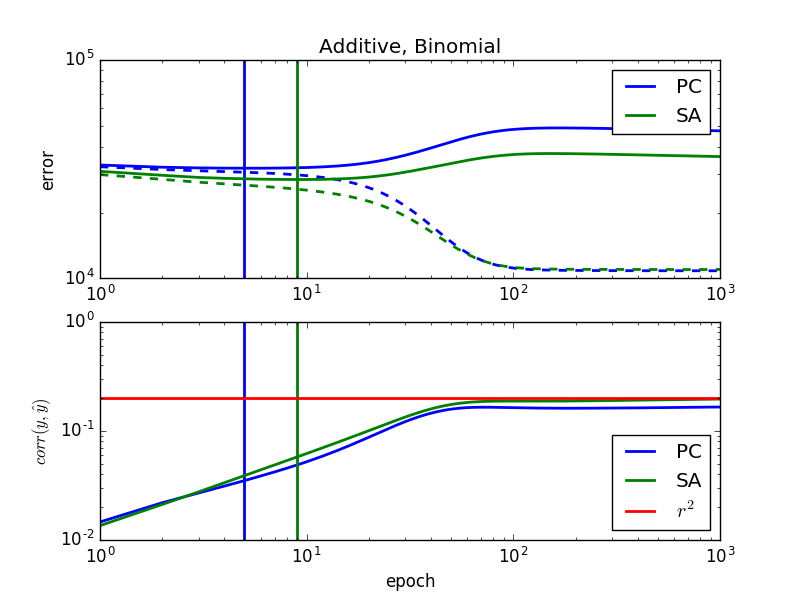
\includegraphics[width=0.4\textwidth]{img/add_gsu}
  \caption{Simulation: Additive Effect, $r^2 = 0.2$ }
  \label{fig:simu1}
\end{figure}
\begin{figure}[h]
  \centering
  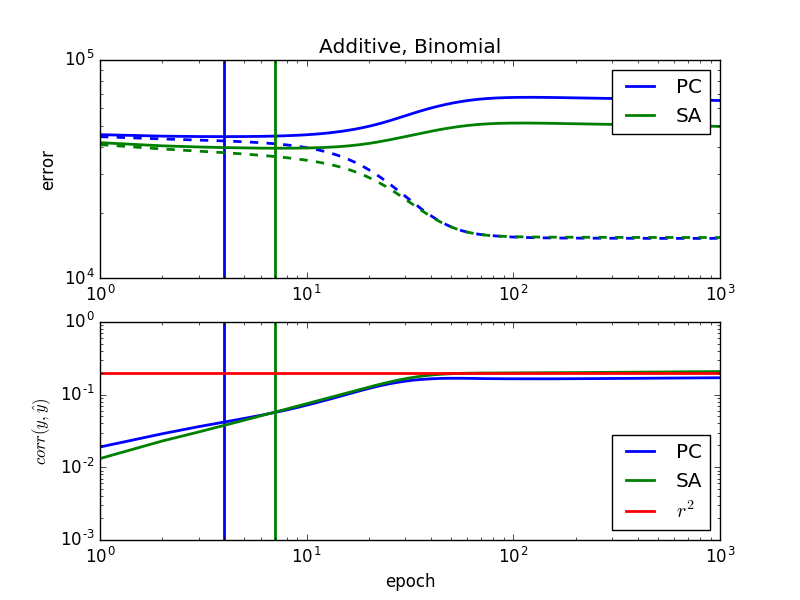
\includegraphics[width=0.4\textwidth]{img/cmp_gsu}
  \caption{Simulation: Composite Effect, $r^2 = 0.2$ }
  \label{fig:simu2}
\end{figure}
Both figure (\ref{fig:simu1}) and (\ref{fig:simu2}) show that networks trained using intermediate features extracted by SAs ($\bs{h}_1$, solid solid green) exhibits lower testing error than the first principle component ($\bs{h}_1^\prime$, solid blue), which is in support of the existence of non-linear relationship among raw features, because we expect the two share similar performance if the raw features only linearly correlated, in which case PCA should adequately remove redundancies with the super-blocks. In addition, if we transform the y axis back from log scale, the gap between the two testing errors are larger in the composite effect scenario (Figure \ref{fig:simu2}) than the the one in the additive genetic effect scenario (Figure \ref{fig:simu1}), which is in support of the proposed hypothesis that ``missing heritability'' can be attributed to non-linear link between genomic features and the phenotype.

In terms of $corr(\bs{y}, \hat{\bs{y}})$ though, features extracted by SAs and PCA demonstrate compatible convergence, both of which went close to $r^2 = 0.2$ -- is the theoretical upper limit pre-specified by the simulation, in a similar pace. However, the former show a slight edge over the later after convergence in both scenarios.

Other interesting observations are the emergence of over-fitting and the early stop rule. The training error of both type of input features showed over-fitting after a certain number of iterations, if we decide to stop training at the lowest possible testing error (shown in vertical bars), the over-fitting can be avoided, yet the prediction - truth shows plenty room for improvement. It seem a better stopping rule should rely on detecting the stagnation of correlation, instead of the rising of testing error. In fact, one would better off letting the model overfit for a small number of epochs.

\section{Body Height Data analysis}
The correlation between predicted value and true value in testing set is used as criteria to evaluate performance. Results for different network settings can be found at Figure (\ref{fig:real1}). For different activation functions, we can see that all activation functions over-fits the data very quickly, usually after 2 epochs. We claim it is due to large sample size and relatively small batch size (64) such that in one epoch (iterate through all the 80K samples), the model already updates the gradient for thousands of times. Another reason could be the simple mechanism of association between height and features which implies height is a highly additive trait and the effect that features have on height is simple and mostly linear. Moreover, linear activation function outperforms all the other activation functions, even after over-fitting. The nonlinear activation functions fail to capture the assumed nonlinear association. Larger sample size directly improves prediction accuracy. For learning rate, smaller learning rate slows down over-fitting procedure. A good way to deal with over-fitting is to add regularization terms. Here we used $l_0$ penalty and evaluate performance under different cases. We can see from result that larger $\lambda$ offer protection against over-fitting, and with large sample size, prediction accuracy is maintained under different scenarios.
\begin{figure}[h]
  \centering
  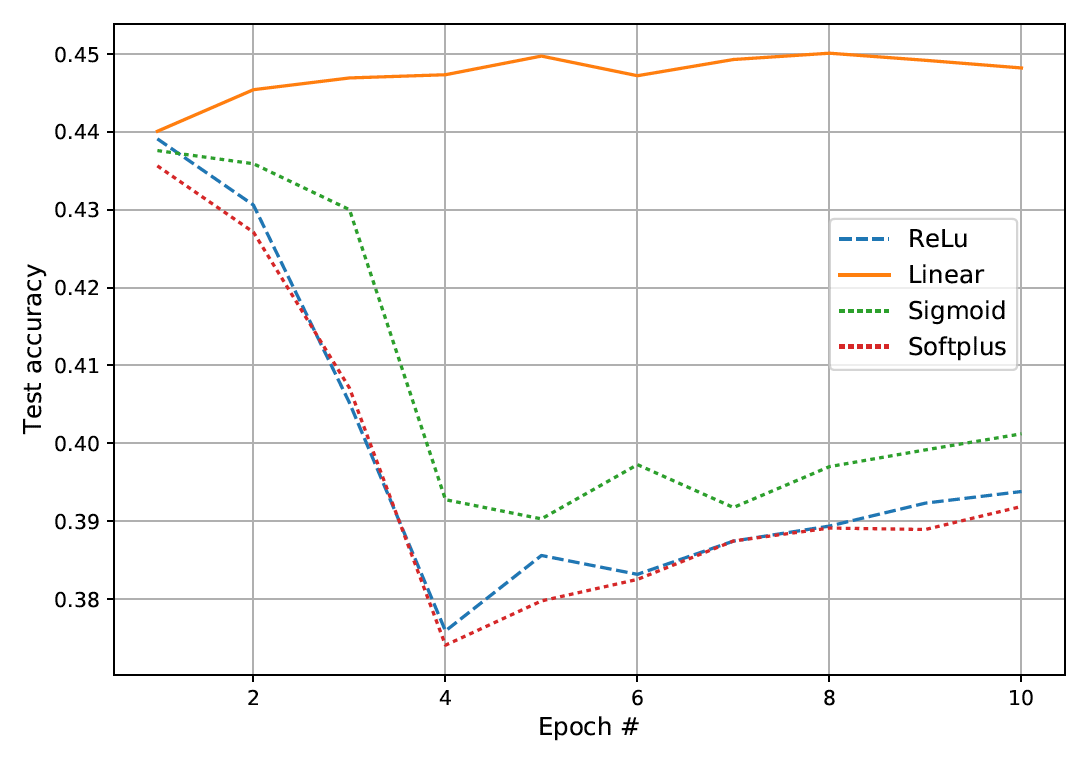
\includegraphics[width=0.23\textwidth]{img/acc_vs_activation}
  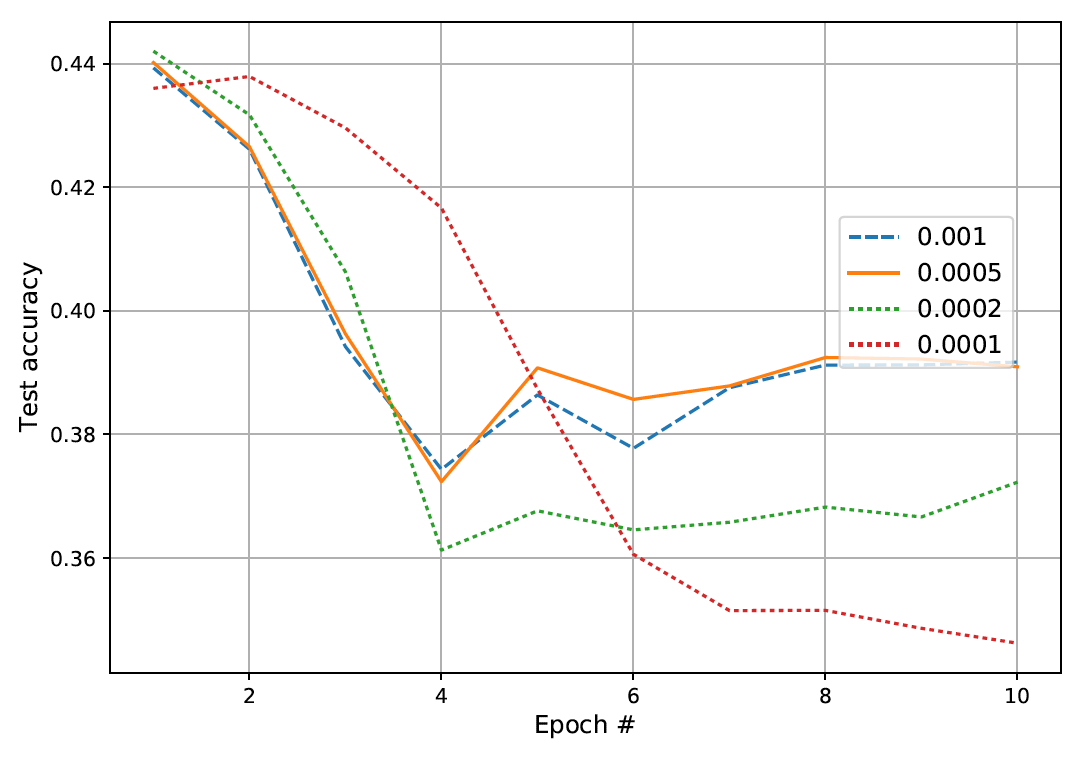
\includegraphics[width=0.23\textwidth]{img/acc_vs_lr} \\
  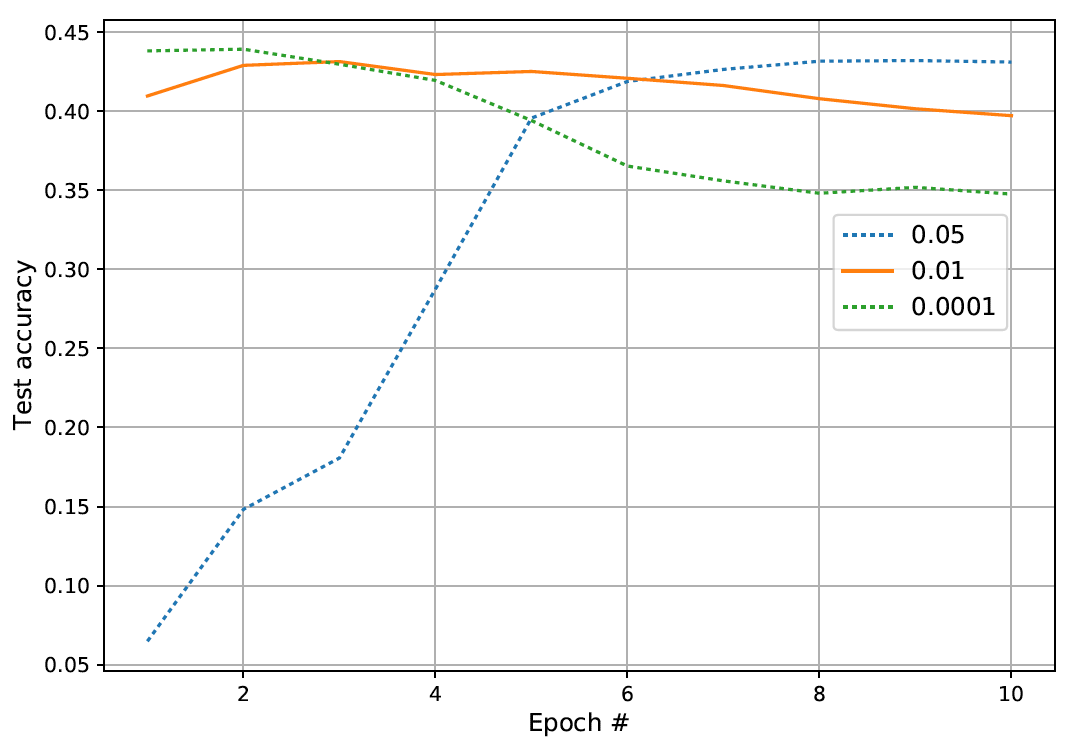
\includegraphics[width=0.23\textwidth]{img/acc_vs_reg}
  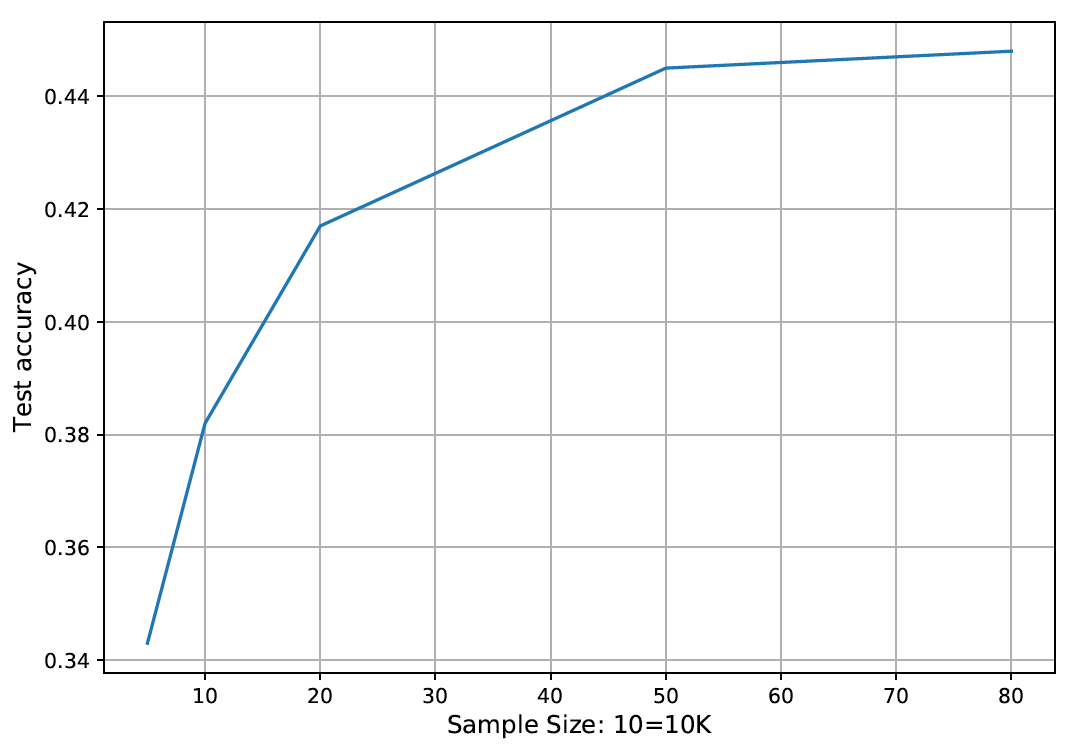
\includegraphics[width=0.23\textwidth]{img/acc_vs_samplesize}
  \caption{UK Biobank Height Data Analysis}
  \label{fig:real1}
\end{figure}
The final prediction accuracy for different selected feature sets under different methods can be found at Table (\ref{tab:pred1}). A highest prediction accuracy is achieved by Bayesian generalized linear models on top-p value selection with 45.9\% prediction accuracy. Step-wise selection achieves slightly lower accuracy of 45.7\% under BGLM methods. The results shows: i) selected features works much better than random picked features which indicates effectiveness of variable selection. ii) the generative models works better than neural networks for height trait. the neural network fails to capture nonlinear association between features and trait. iii) For neural network linear activation function outperforms other activation functions. iv) Step-wise selection does not outperform top-p value selection.

\begin{table}[h!]
\centering
\caption{Prediction Accuracy}
\label{tab:pred1}
\begin{tabular}{|c|c|c|c|}
\hline
                & NN(Linear) & NN(ReLU) & BGLM  \\ \hline
Random, 6K      & 0.137      & 0.140    & 0.161 \\ \hline
Top P value, 6K & 0.452      & 0.442    & 0.459 \\ \hline
Block BIC, 6K   & 0.449      & 0.440    & 0.457 \\ \hline
\end{tabular}
\end{table}

% Bibliography
\bibliographystyle{ACM-Reference-Format}
\bibliography{ref}

\end{document}
